\chapter{Конструкторская часть}

В этом разделе разработаны структура данных словаря, алгоритм бинарного поиска в словаре и алгоритм определения соответствия введённого запроса распознаваемым вариантам. Также будут представлены схемы данных алгоритмов.

\section{Разработка алгоритма бинарного поиска в словаре}
На рисунке \ref{img:bin} представлена схема реализации алгоритма бинарного поиска в словаре. 

\begin{figure}[h!]
    \centering
    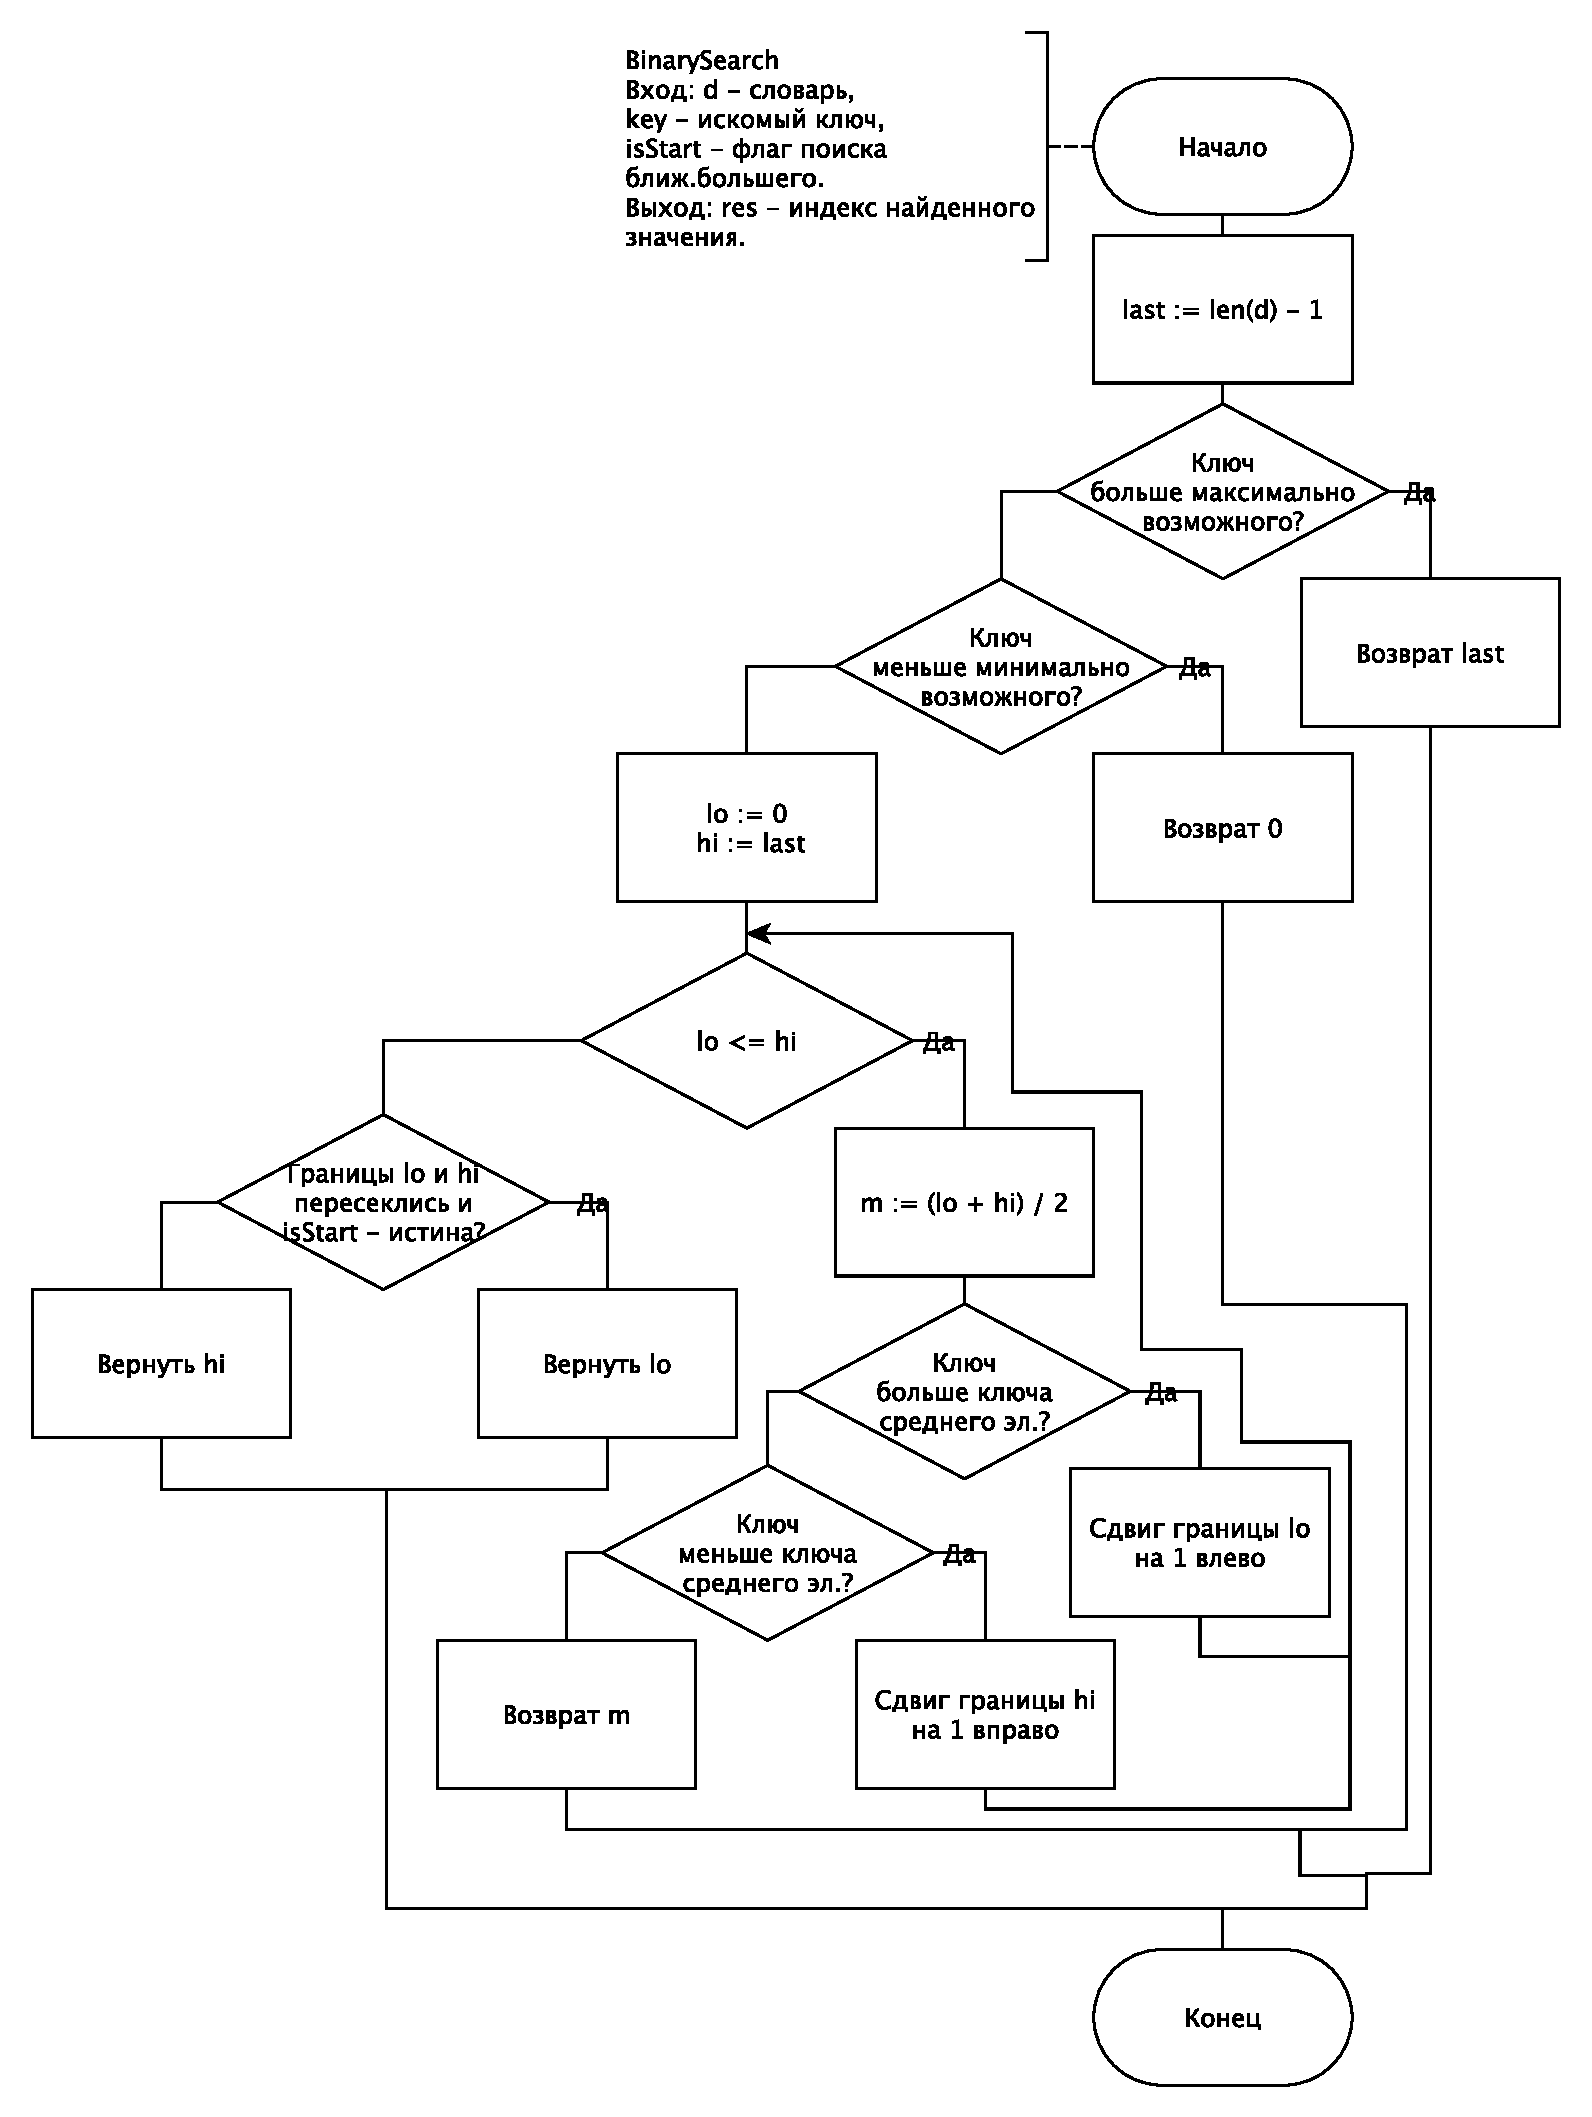
\includegraphics[width=0.65\linewidth]{bin.pdf}
    \caption{Схема реализации алгоритма бинарного поиска в словаре}
    \label{img:bin}
\end{figure}

\section{Разработка алгоритма определения соответствия введённого запроса распознаваемым вариантам}
На рисунке \ref{img:recogn} представлена схема реализации алгоритма определения соответствия введённого запроса распознаваемым вариантам.

\begin{figure}[h!]
    \centering
    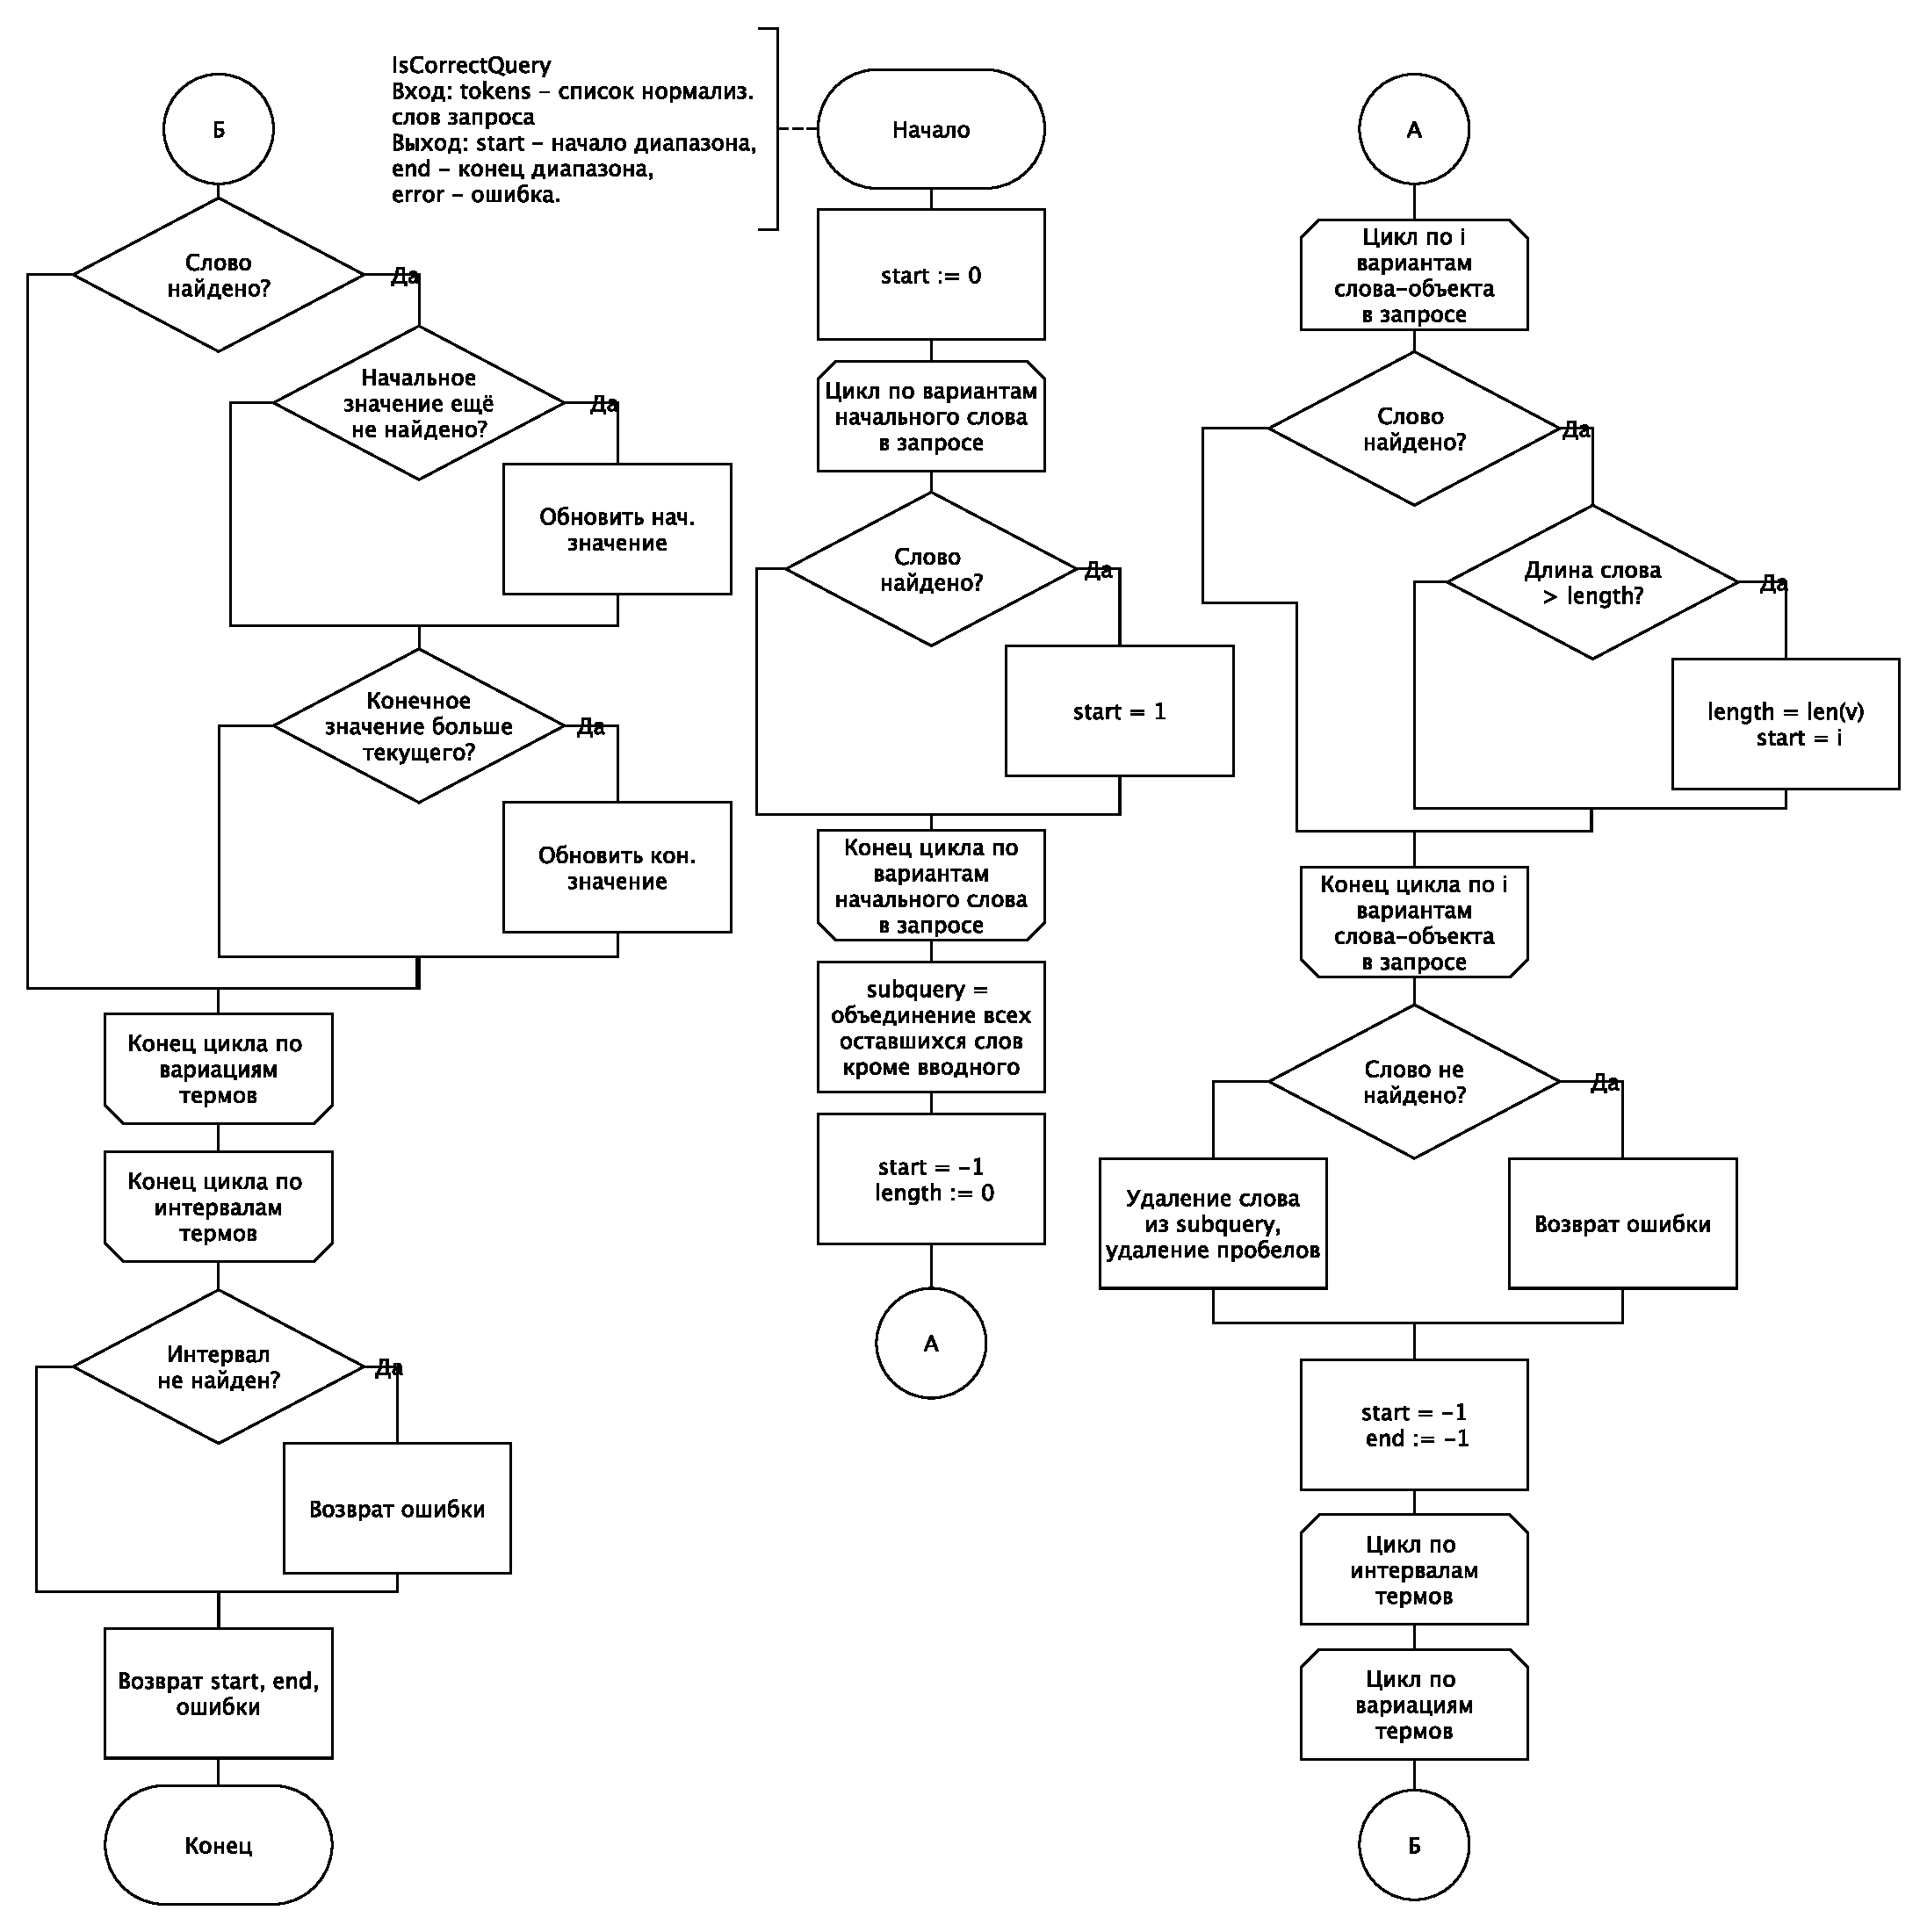
\includegraphics[width=1\linewidth]{recogn.pdf}
    \caption{Схема реализации алгоритма определения соответствия введённого запроса распознаваемым вариантам}
    \label{img:recogn}
\end{figure}

\section{Разработка структуры данных словаря}
Было принято решение подразумевать под структурой словаря массив $Dictionary$ записей $Word$ формата «ключ-значение», где ключом $key$ словаря является количество шерсти у кошки на см$^2$ тела, а значением $value$ является структура, хранящая информацию о породе кошки, её пушистости и ссылку на изображение кошки.

\newpage